\section{Einleitung}
\label{sec:einleitung}

Das Softwareprojekt \emph{Common Unfolding} entstand im Sommersemester 2011 im Rahmen der Veranstaltung \emph{Softwareprojekt: Anwendungen von Algorithmen} unter Leitung von Herrn Prof. Dr. Rote. Es entstand ein Programm, mit dessen Hilfe, auf zeichnerischem Wege Polygone gefunden werden können, aus denen zwei verschieden Quader \bzw Schachteln gefaltet werden können. Im Folgenden wird die genaue Problemstellung näher erläutert, sowie die Zielstellung unseres Projektes definiert.


%%%%%%%%%%%%%%%%%%%%%%%%%%%%%%%%%%%%%%%%%%%%%%%%%%%%%%%%%%%%%%%%%%%%%%%%%%%%%%%
%%%%%%%%%%%%%%%%%%%%%%%%%%%%%%%%%%%%%%%%%%%%%%%%%%%%%%%%%%%%%%%%%%%%%%%%%%%%%%%
%%%%%%%%%%%%%%%%%%%%%%%%%%%%%%%%%%%%%%%%%%%%%%%%%%%%%%%%%%%%%%%%%%%%%%%%%%%%%%%
% PROBLEMSTELLUNG UND AUFGABENSTELLUNG %%%%%%%%%%%%%%%%%%%%%%%%%%%%%%%%%%%%%%%%
%%%%%%%%%%%%%%%%%%%%%%%%%%%%%%%%%%%%%%%%%%%%%%%%%%%%%%%%%%%%%%%%%%%%%%%%%%%%%%%
\subsection{Problemstellung und Aufgabenstellung}
\label{subsec:problemstellung}

Grundsätzlich geht es um das Falten von orthogonalen Polygonen zu Quadern \bzw Schachteln. Unter orthogonalen Polygonen versteht man Polygone, die ausschließlich Innenwinkel mit 90$^\circ$ oder 270$^\circ$ besitzen. Beispielsweise ist das Netz eines Würfles ein orthogonales Polygon (siehe Abb.~\ref{fig:polygon}).

\begin{figure}[htbp]
\centering
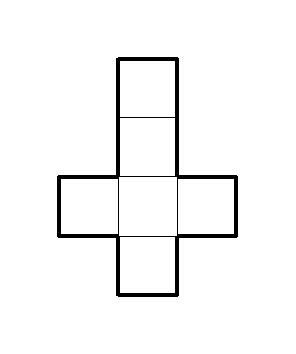
\includegraphics{03_pics/polygon.pdf}
\caption{Orthogonales Polygon}
\label{fig:polygon}
\end{figure}

Es existieren orthogonale Polygone als Grundfläche, welche, auf unterschiedliche Arten, \dH an verschiedenen Kanten gefaltet, in zwei verschieden dimensionierten Quadern resultieren. Dieses Polygon wird als \emph{common unfolding}~\cite{commonUnfold} der Quader bezeichnet. In Abbildung \ref{fig:Common-Unfolding} ist ein Beispiel einer Grundfläche gezeigt, aus welcher zwei verschiedene Schachteln in den Dimensionen $1\times2\times3$ und $1\times1\times5$ gefaltet werden können. Da beide Schachteln aus dem selben Polygon gefaltet wurden, haben sie identische Oberflächeninhalte.

\begin{figure}[htbp]
\centering
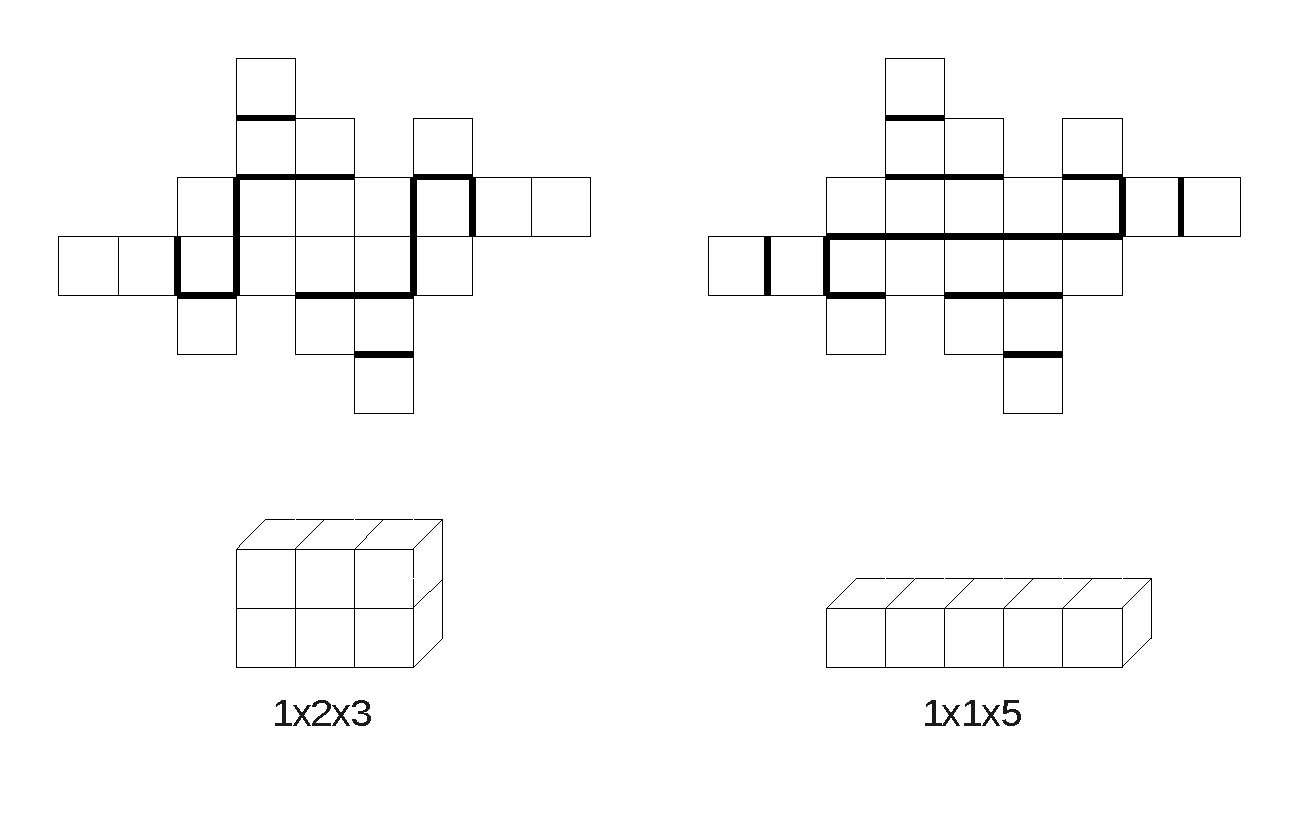
\includegraphics[scale=0.5]{03_pics/commonUnfold_beispiel1.pdf}
\caption{Common Unfolding}
\label{fig:Common-Unfolding}
\end{figure}

Um solche Grundflächen (common unfoldings) zu finden, war es unsere Aufgabe ein Programm zu entwickeln, welches eine zeichnerische Lösung des Problems ermöglicht. Zur Lösungsfindung wird die Idee des \emph{Simultanen Zeichnens} verwendet. Unter simultanem Zeichnen versteht man das gleichzeitige Zeichnen auf mehreren Grundflächen \bzw aufgefalteten Gitternetzen, siehe Abbildung~\ref{fig:Simpultanes-Zeichnen}. Ausgangspunkt sind dabei zwei (oder mehr) Quader mit verschiedenen Kantenlängen, aber gleichem Flächeninhalt. Für diese Quader soll nun, falls existent, das common-unfold Polygon gefunden werden. Auf den Oberflächen der Quader, wird gleichzeitig gezeichnet. Genauer gesagt ist die Oberfläche der Quader in beliebig kleine Flächenstücke eingeteilt, welche \emph{ausgemalt} werden. Wir erhalten die Lösung, wenn alle gegeben Quaderoberflächen komplett ausgemalt sind. Die Stellen an denen die Schachtel gefaltet werden soll, muss selbständig gefunden werden, eine Lösung dafür wird durch das Programm nicht geliefert. 


\begin{figure}[htbp]
\centering
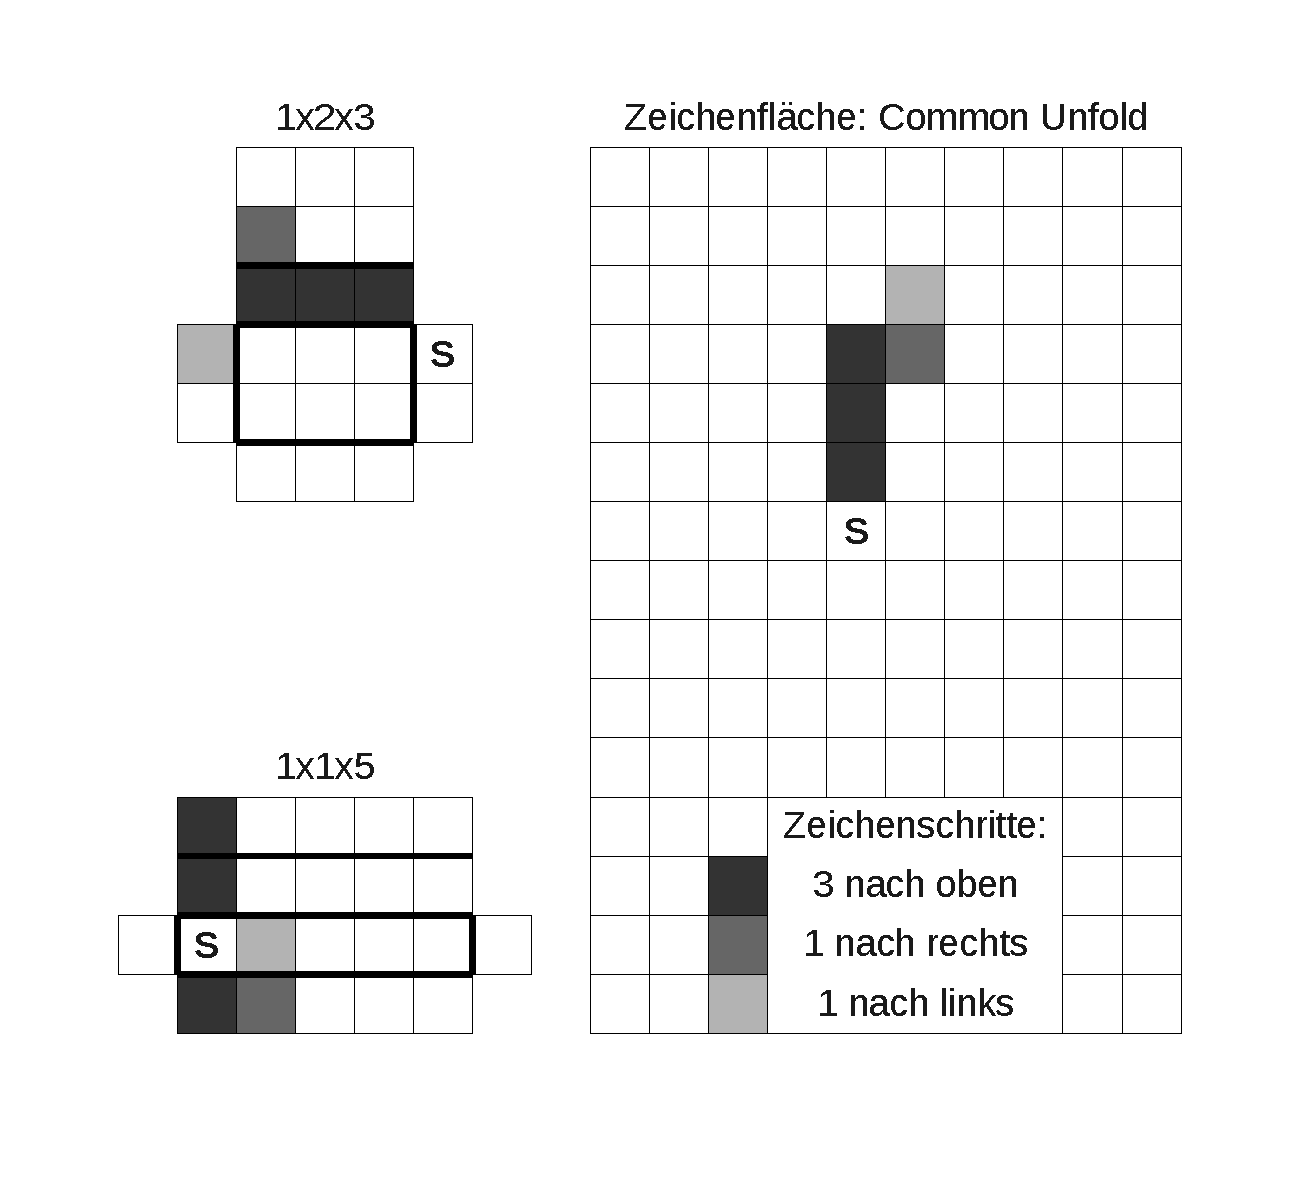
\includegraphics[scale=0.5]{03_pics/simulatnes_zeichnen.pdf}
\caption{Simpultanes Zeichnen}
\label{fig:Simpultanes-Zeichnen}
\end{figure}


%%%%%%%%%%%%%%%%%%%%%%%%%%%%%%%%%%%%%%%%%%%%%%%%%%%%%%%%%%%%%%%%%%%%%%%%%%%%%%%
%%%%%%%%%%%%%%%%%%%%%%%%%%%%%%%%%%%%%%%%%%%%%%%%%%%%%%%%%%%%%%%%%%%%%%%%%%%%%%%
%%%%%%%%%%%%%%%%%%%%%%%%%%%%%%%%%%%%%%%%%%%%%%%%%%%%%%%%%%%%%%%%%%%%%%%%%%%%%%%
% ZIELE UNSERES PROJEKTS %%%%%%%%%%%%%%%%%%%%%%%%%%%%%%%%%%%%%%%%%%%%%%%%%%%%%%
%%%%%%%%%%%%%%%%%%%%%%%%%%%%%%%%%%%%%%%%%%%%%%%%%%%%%%%%%%%%%%%%%%%%%%%%%%%%%%%
\subsection{Ziele unseres Projekts}
\label{subsec:ziele}

Das Ziel unseres Softwareprojektes war es, ein Programm zu entwickeln, welches eine 2D grafische Benutzeroberfläche bietet, um solche \emph{common unfolding}-Polygone zu finden. Das Programm sollte eine flexible Auswahl der Startquader bieten und den zeichnerischen Vorgang, also das gleichzeitige Zeichnen auf mehreren Schachtel ermöglichen.

\newpage


%%%%%%%%%%%%%%%%%%%%%%%%%%%%%%%%%%%%%%%%%%%%%%%%%%%%%%%%%%%%%%%%%%%%%%%%%%%%%%%
%%%%%%%%%%%%%%%%%%%%%%%%%%%%%%%%%%%%%%%%%%%%%%%%%%%%%%%%%%%%%%%%%%%%%%%%%%%%%%%
%%%%%%%%%%%%%%%%%%%%%%%%%%%%%%%%%%%%%%%%%%%%%%%%%%%%%%%%%%%%%%%%%%%%%%%%%%%%%%%
% GLIEDERUNG %%%%%%%%%%%%%%%%%%%%%%%%%%%%%%%%%%%%%%%%%%%%%%%%%%%%%%%%%%%%%%%%%%
%%%%%%%%%%%%%%%%%%%%%%%%%%%%%%%%%%%%%%%%%%%%%%%%%%%%%%%%%%%%%%%%%%%%%%%%%%%%%%%
\subsection{Gliederung der Arbeit}
\label{subsec:gliederung}
Der Abschlussbericht ist wie folgt strukturiert: Zunächst wird das Projektmanagement in Kapitel~\ref{sec:projektmanagement} erläutert. Dazu gehören die Erfahrungen bezüglich der Zusammenarbeit im Team und der Ablauf des Entwicklungsprozesses.\\

In Kapitel~\ref{sec:frontend} wird das User Interface und die Bedienung des Programms vorgestellt.\\

Eine Beschreibung der Anforderungen und Funktionalität des Programms, sowie der verwendeten \bzw implementierten Algorithmen und Funktionen erfolgt im Kapitel~\ref{sec:backend}: Softwarearchitektur. Dabei werden Schwierigkeiten und Herausforderungen bezüglich der Implementierung dargelegt und Verbesserungsmöglichkeiten aufgezeigt.\\

Schließlich erfolgt in Kapitel~\ref{sec:zusammenfassung} eine Zusammenfassung der Projektergebnisse und der erreichten Ziele. Außerdem werden unsere gewonnen Erkenntnisse \bzw "`Was haben wir dabei gelernt?"' dargelegt und ein Ausblick auf zukünftige Arbeiten gegeben.

